\documentclass[11pt]{report}
\setcounter{tocdepth}{3} %shows all levels incl. paragraph
\usepackage[spanish]{babel}
\usepackage[tmargin=1in,bmargin=1in,lmargin=1.25in,rmargin=1.25in]{geometry}
\usepackage[T1]{fontenc}
\usepackage{graphicx}
\usepackage[usenames]{color}
\usepackage{amssymb}
\usepackage{amsmath} 
\usepackage{hyperref}
\usepackage{graphicx}
\usepackage[utf8]{inputenc}
\usepackage{booktabs}
\usepackage{listings}
\usepackage{pdflscape}
\newcommand{\tabitem}{~~\llap{\textbullet}~~}
\renewcommand{\contentsname}{Índice}
\usepackage{array}
%%Jawascript definition
\usepackage{color}
\definecolor{lightgray}{rgb}{.9,.9,.9}
\definecolor{darkgray}{rgb}{.4,.4,.4}
\definecolor{purple}{rgb}{0.65, 0.12, 0.82}
\lstdefinelanguage{Javascript}{
  keywords={typeof, new, true, false, catch, function, return, null, catch, switch, var, if, in, while, do, else, case, break},
  keywordstyle=\color{blue}\bfseries,
  ndkeywords={class, export, boolean, throw, implements, import, this},
  ndkeywordstyle=\color{darkgray}\bfseries,
  identifierstyle=\color{black},
  sensitive=false,
  comment=[l]{//},
  morecomment=[s]{/*}{*/},
  commentstyle=\color{purple}\ttfamily,
  stringstyle=\color{red}\ttfamily,
  morestring=[b]',
  morestring=[b]"
}

\lstset{
   language=JavaScript,
%   backgroundcolor=\color{lightgray},
   extendedchars=true,
   basicstyle=\footnotesize\ttfamily,
   showstringspaces=false,
   showspaces=false,
%   numbers=left,
%   numberstyle=\footnotesize,
%   numbersep=9pt,
   tabsize=2,
   breaklines=true,
%   showtabs=false,
   captionpos=b
}



\author{[Technical Report]}
\author{Jimenez García Eduardo Gamaliel\and Ortiz Chávez Alejandro\and Resendiz Arteaga Juan Alberto}

\begin{document}
  %%  COVER
\pagenumbering{Alph}
\begin{titlepage}
    \begin{center}
    \begin{tabular}{r c l}
    
\includegraphics[scale=.20]{images/ipn} & \textbf{INSTITUTO POLIT\'ECNICO NACIONAL} & 
\includegraphics[scale=.20]{images/escom}\\ 
    & \textbf{ESCUELA SUPERIOR DE C\'OMPUTO}
    \end{tabular}
    \end{center}


    \vspace{1.5cm}
    \begin{center}
    \large Trabajo Terminal: \linebreak

    \large \textbf{``Ambienta2MX''} \linebreak
    \large 2014B-073

    \end{center}

    \vspace{1.5cm}

    \begin{center}
    Presentan: \linebreak
    \textbf{Jimenez García Eduardo Gamaliel} \linebreak
    \textbf{Reséndiz Arteaga Juan Alberto} \linebreak
    \end{center}

    \vspace{1.5cm}


    %En el presente documento se encuentran los resultados correspondientes al desarrollo del Trabajo Terminal cuyo objetivo es la implementaci\'on de un sistema que analice mensajes mediante  procesamiento de lenguaje natural y teoría de reconocimiento de patrones. Este sistema pretende servir como herramienta capaz de clasificar la intención de dichas  conversaciones como peligrosas o no peligrosas. \linebreak

    \textbf{Palabras Clave}:  Desarrollo Web, Sistemas distribuidos, Aplicaciones para las comunicaciones en red.

    \vspace{1.5cm}
     
    \begin{center}


    Directores: \linebreak
    \textbf{ M. en C. Ram\'irez Morales Mario Augusto, M. en E.  Silva S\'anchez Carlos}

    \end{center}
\end{titlepage}
\pagenumbering{arabic}
  \tableofcontents

  \chapter*{Introducción}
\addcontentsline{toc}{chapter}{Introducción}
	\paragraph{\underline{Ambienta2MX} pretende ser una plataforma única en su tipo a nivel nacional, proporcionando la infraestructura lógica, modelo de datos, diagramas y esquemas lógicos necesarios para proveer un servicio de consulta de datos climatologicos e índices de contaminación a través de un portal web y/o servicios expuestos, para fines privados, públicos o sociales en general.}
    \paragraph{Han existido diversos diversos sistemas que proveen información semejante o han intentado dar solución a la problemática expuesta no solo considerando datos ambientales cómo la temperatura sino geográficos, geodésicos, topográficos, etcetera; sin embargo, no han tenido el impacto o el apoyo necesario para crecer y proveer la infraestructura lógica y/o física para satisfacer ese problema.}
    \paragraph{Para llegar a la solución que será descrita a lo largo de éste documento fue necesario considerar un grupo específico de soluciones existentes, que van desde sistemas totalmente orientados a la estandarización, hasta soluciones que toman sólo parte del problema completo que pretende atacar Ambienta2MX.}
    \paragraph{Problemas de este tipo han sido atacados en otros países, teniendo un impacto favorable en la consulta de información de cierta área en específico, casos como el anterior serán mencionados próximamente.}

  \chapter {Antecedentes}
\section {Sistemas de información geográfica}
  \paragraph {Un Sistema de Información Geográfica (GIS, por sus siglas en inglés) es un sistema computacional de captura, almacenamiento, chequeo y exposición de datos relacionados a la superficie de la Tierra. Los SIG pueden mostrar información de varios tipos en un mismo lienzo (usualmente mapas) lo que facilita el análisis de la información recolectada.\cite{5}}

  \paragraph{Los SIGs son una herramienta usada por organizaciones, escuelas, instituciones gubernamentales y negocios. Éstos sistemas pueden ser orientados a datos globales o a una región en específico del globo terraqueo. Entre los datos almacenados más importantes se encuentra la georeferenciación (Longitud, Latitud, Altitud), algunos datos relativos a la zona, por ejemplo, códigos postales.}

  \begin{figure}[h!]
      \centering
        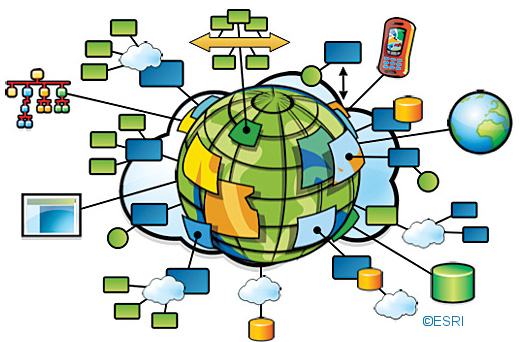
\includegraphics[width=\textwidth]{./images/GIS.jpg}
      \caption{Sistemas de Información Geográfica. \cite{18}}
  \end{figure}

  \paragraph{En México, la institución encargadada del manejo de datos estadíticos y geográficos es el INEGI. El Instituto Nacional de Estadística, Geografía e Informática (INEGI) es la fusión de varias instituciones gubernamentales que funcionaban de forma independiente hasta el año 1983; éstas se encargaban de el manejo de datos estadísticos, comerciales, económicos y financieros.}

  \paragraph{Actualmente el INEGI, sede se encuentra ubicada en Aguascalientes, Aguascalientes, es la institución encargada de la captación, procesamiento y difusión de información relativa al territorio nacional. \cite{6}}

  \paragraph{Los datos geoespaciales (Longitud, Latitud, Altitud) que brinda el INEGI se encuentran bajo el estandar \textbf{ITRF 2008} en época 2010. Sin embargo, aún existen sistemas que se encuentran trabajando bajo el formato ITRF92 época 1988 y NAD27 (formato usado hasta 1998), para ello, se brindará soporte a formatos previos, dando prioridad al último estandar existente.} 

\section {Sistemas de Monitoreo del medio Ambiente.}
  \subsection {Proyecto en la ciudad de Salamanca}
    \paragraph {Uno de los proyectos nacionales que realizo un monitoreo usando un PCFM fue realizado en la ciudad de Salamanca- una de las ciudades más contaminadas en México. Este proyecto es titulado “Análisis de la contaminación del aire usando un Algoritmo PCFM  aplicado a una base de datos real.}

    \paragraph{La intención del estudio es analizar la relación entre contaminación y las variables ambientales. En el análisis de este estudio se involucraron datos desde Enero a Diciembre del 2007. Algunas de las variables que se incluyeron fueron S02, y la concentración de partículas menores a 10m y variables meteorológicas. Velocidad del viendo, dirección del viento, temperatura y humedad relativa. A partir de este estudio se instalaron algunos centros de monitoreo en Salamanca.}

  \subsection {Inventario Nacional de Emisiones de Gases de Efecto Invernadero (INEGEI)}
    \paragraph {En este proyecto se elabora un informe que comprende las estimaciones de las emisiones por fuente y sumidero. Esto se realiza de acuerdo a lo conforme establecido en los artículos 4 y 12 de la Convención marco de las naciones unidas sobre el cambio climático. Este proyecto es una publicación que nos ayuda a saber que deficiencias tenemos, y que efectos pudiera llegar a tener el exceso de algunos contaminantes, sin embargo no es una plataforma para accede a estos datos tan importantes.}

  \subsection {Mapa Digital -  INEGI}
    \paragraph {Este proyecto es un sistema de información geográfica que tiene como objetivo facilitar el estudio de los objetos geográficos a través del conocimiento de su ubicación espacio-temporal, así como de atributos asociados;  tales servicios bridan al usuario final la posibilidad de:}

  \begin{itemize}
    \item {Mostrar en forma gráfica la dimensión de la información contenida por medio de acercamientos, selección de capas de información, localizaciones, mediciones, etc.}
    \item {Analizar e interpretar los contenidos geográficos y estadísticos mediante operaciones matemáticas, mapas temáticos, gráficos estadísticos, análisis espacial y estadísticos básicos.}
    \item {Integrar información a través de la incorporación de datos vectoriales y raster provenientes de archivos locales, conexiones a servicios WMS y base de datos geospaciales de PostGis.}
  \end{itemize}

  \paragraph{Toda la información que muestra el mapa digital del INEGI es obtenida por medio de servicios tipo REST, se puede hacer uso de éstos usando Web Scrapping, sin embargo, se encuentra totalmente ligado a la aplicación, trayendo consigo problemas en caso de que se deseara extraer el contenido que ofrecen.}

  \begin{figure}[h!]
      \centering
        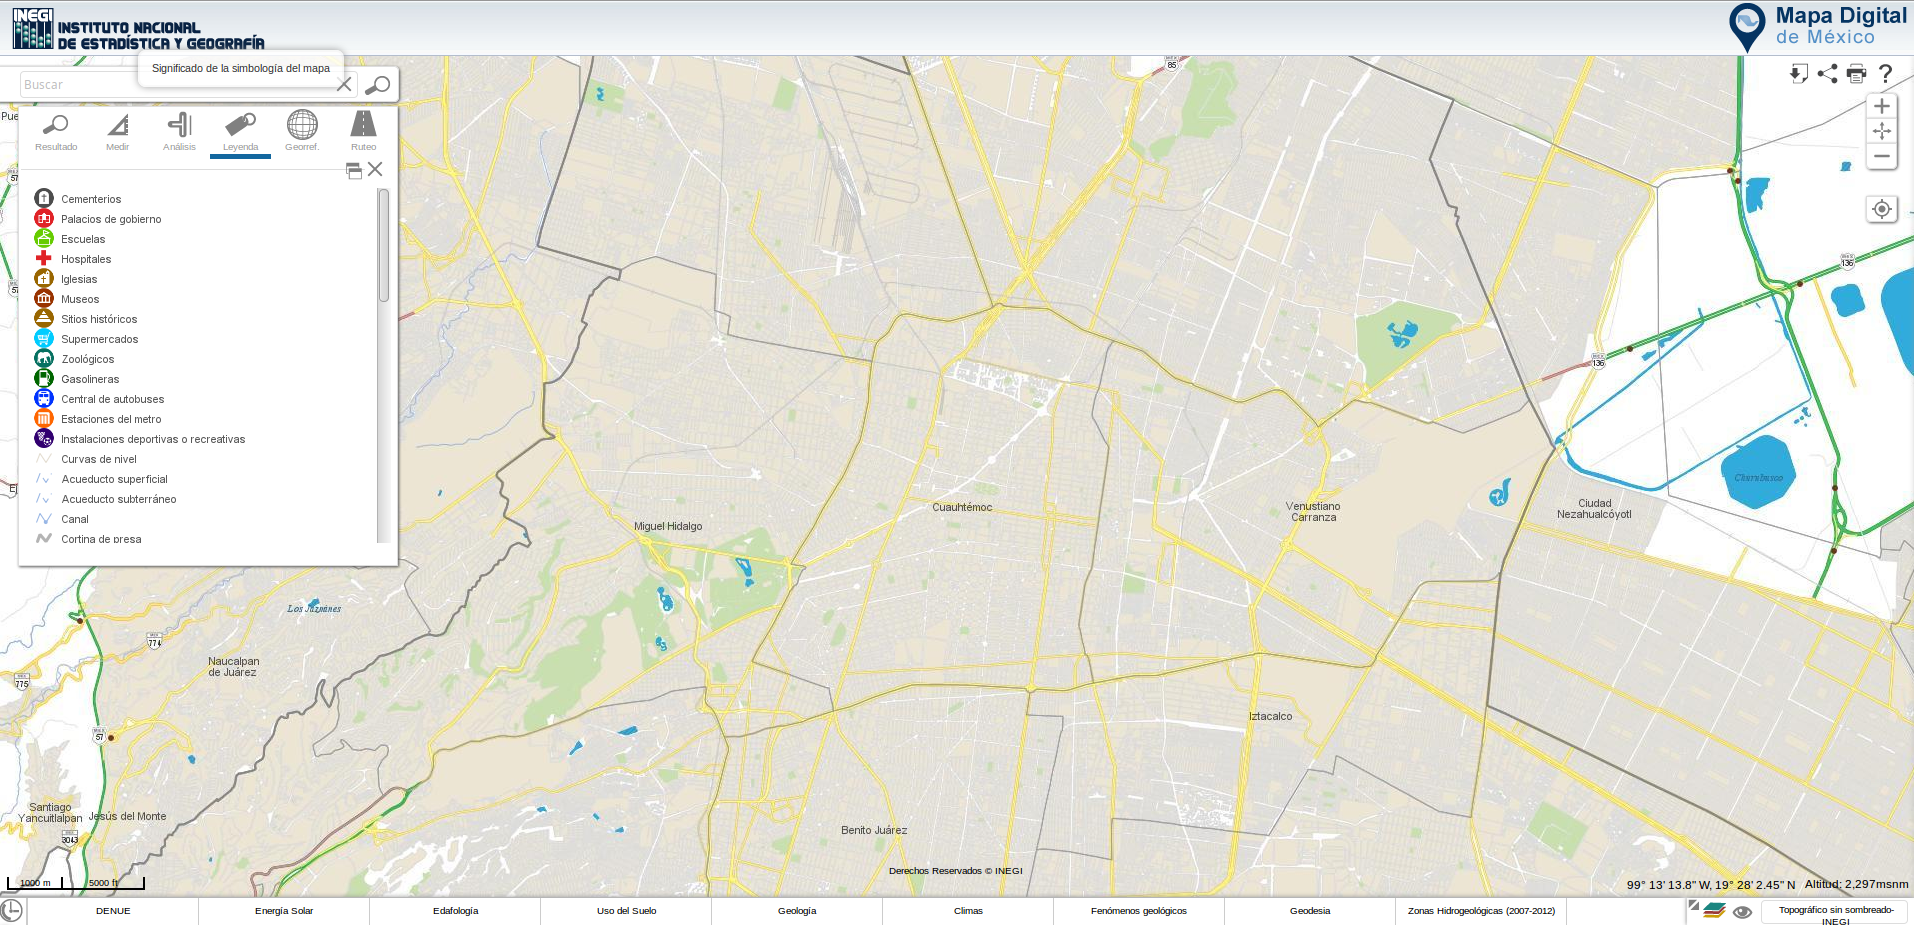
\includegraphics[width=\textwidth]{./images/MapaDigital.png}
      \caption{Mapa Digital - INEGI.}
  \end{figure}

  \paragraph{El INEGI y el mapa digital cuentan con algunos puntos de acceso a la información usando como medio principal las peticiones HTTP. Estos servicios suelen ser aislados y requieren de una interacción directa con el humano, es decir, es necesario que éste tenga una interacción mediante escritura o clicks en los formularios de éstos.}

  \subsection {Base de Datos Estadísticos BADESNIARN}
    \paragraph {Proyecto de la SEMARNAT que presenta información integrada, revisada y validada con cada una de las fuentes. Además esta estructurada para adecuarse a las necesidades de cada usuario . El usuario en su consulta encontrará el último dato revisado con la fuente, así como la serie histórica disponible en cada caso. Finalmente la plataforma tecnológica detrás le permitirá obtener un archivo electrónica en varios formatos con la info que muestra en pantalla.}    

    \paragraph { Tiene un módulo de consultas temática en donde están muy bien delimitados los temas relacionados con el ambiente, y uno dinámica en donde se asocia cada metadato o archivo con palabras clave para que el usuario pueda encontrar el tema de su interés. \cite{17}}

    \begin{figure}[h!]
        \centering
          
\includegraphics[width=\textwidth]{./images/BADESNIARN.png}
        \caption{Base de datos estadísticos - SEMARNAT.}
    \end{figure}

  \subsection {Forecast IO}
    \paragraph {Es un atlas del clima que se puede visualizar a través de una página web. En el se pueden consultar datos climatológicos – tales como la temperatura actual, probabilidades de precipitación considrando como modo de visualización base mapas de alta definición.}

    \paragraph{Este proyecto integra la información de diversas fuentes y también provee un servicio para obtener datos a través de peticiones REST. Una de sus más grandes desventajas es la limitante de peticiones hacia su servicio, ya que después de cierta cantidad se aplican cargos a una tarjeta definida al dar de alta la cuenta de desarrollador en la plataforma. \cite{14}}

    \begin{figure}[h!]
        \centering
          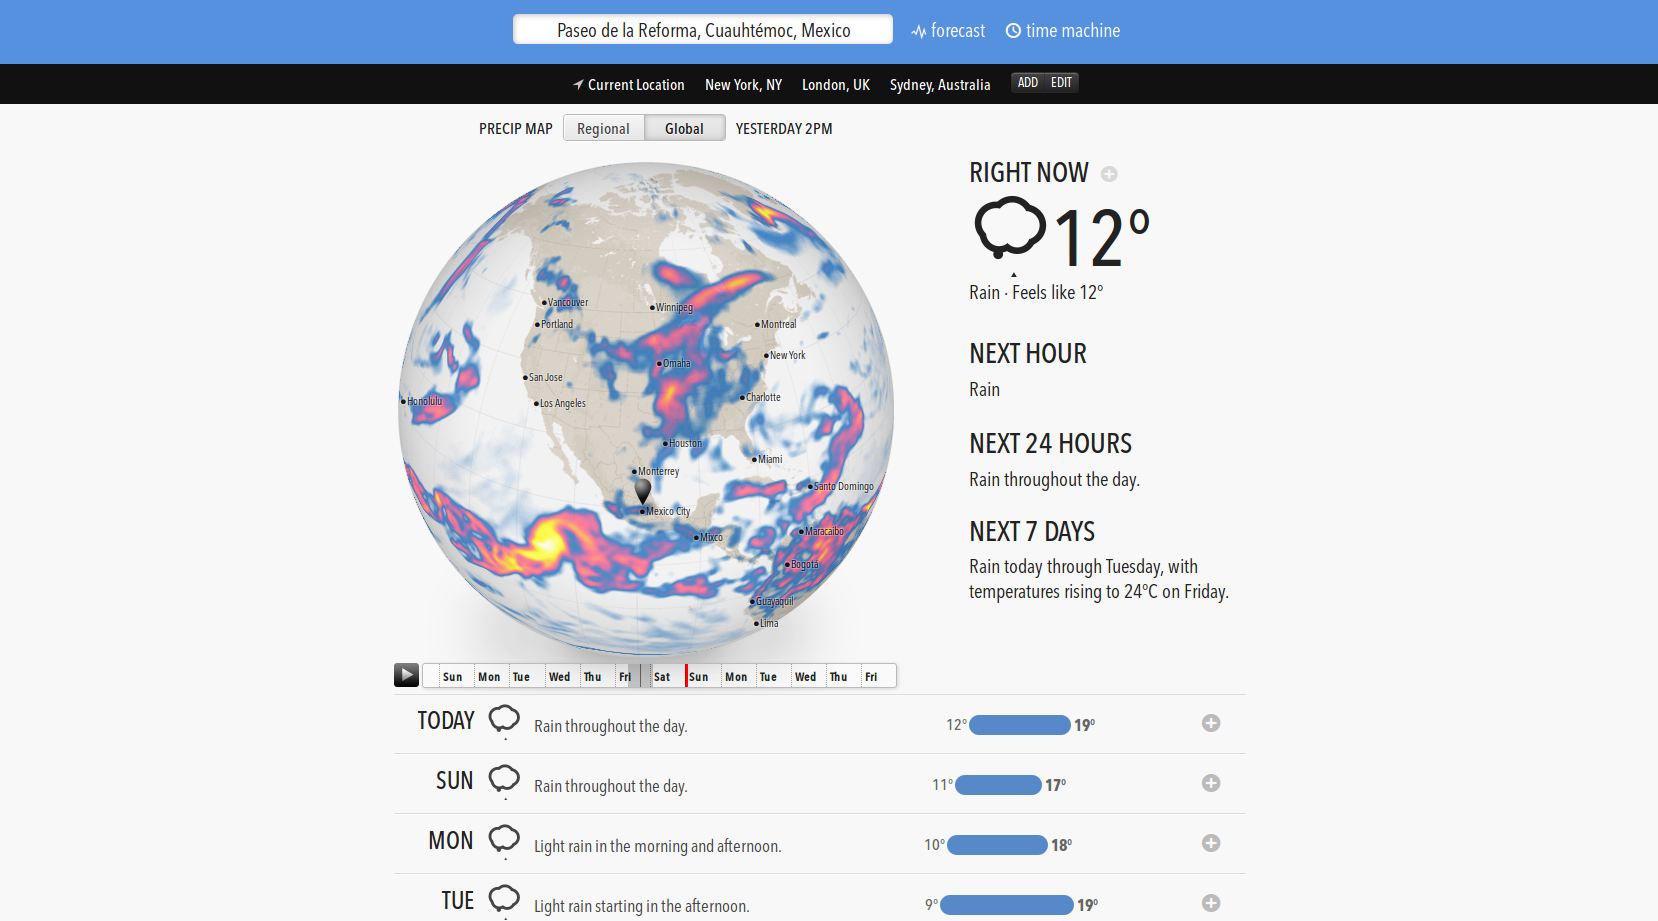
\includegraphics[width=\textwidth]{./images/ForecastIO.png}
        \caption{Forecast.io}
    \end{figure}    

\section{Sistemas de estandarización y unificación de datos.}
  \subsection{Proyecto INSPIRE.}
    \paragraph{El Proyecto INSPIRE comenzó a ser desarrollado el 15 de Mayo 2007 y será completamente implementado para el año 2019. Su principal objetivo es es la creación de una infraestructura única de información geoespacial a lo largo de la unión europea.} 
    \paragraph{La infraestructura de datos espaciales asistirá y trabajará a lo largo de todo el territorio Europeo y parte de Asia(Territorio de perteneciente a Rusia), los datos serán diversos considerando temás comunes y técnicos.}
    \paragraph{El proyecto INSPIRE trabaja bajo algunos principios, por ejemplo:}
    \begin{itemize}
      \item Los datos deben ser recabados sólo una vez y mantenerse actualizados de forma efectiva.
      \item Es posible combinar información espacial de varias fuentes a través del territorio Europeo y compartir sus aplicaciones.
      \item La información geográfica almacenada en todos los niveles será transparente y compartida.
      \item Busqueda fácil de de información geográfica que puede ser usada para fines particulares y de uso general.
    \end{itemize}
    \begin{figure}[h!]
        \centering
          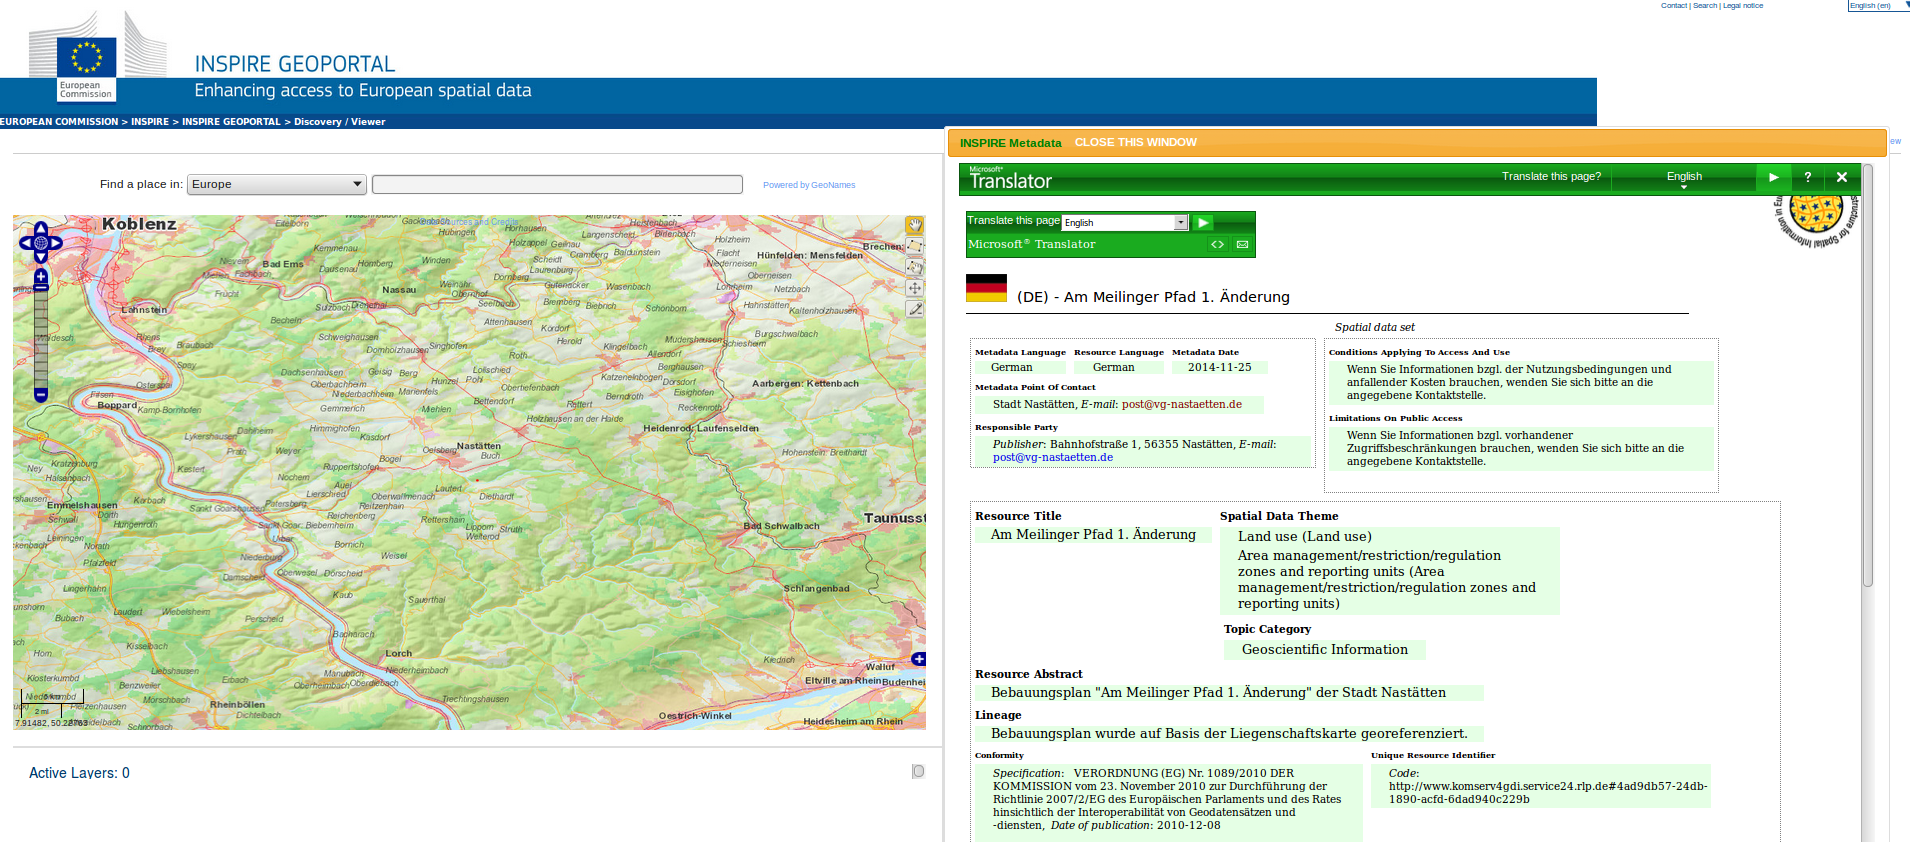
\includegraphics[width=\textwidth]{./images/INSPIRE.png}
        \caption{Visualización de datos y medatados en INSPIRE}
    \end{figure}
    \paragraph{Actualmente parte de los modulos desarrollados se encuentran en etapas de pruebas. Cuenta con un editor de metadatos que consiedera la fecha, el nombre de la organización, correo electrónico, palabras clave, ubicación (Latitud, Longitud, Altitud), entre otros. Los metadatos pueden ser también validados utilizando las mismas herramientas que provee la plataforma.}
    \paragraph{El proyecto INSPIRE cuenta con un proceso de participación de ``StakeHolders'' para mejorar y analizar los detalles específicos del sistema INSPIRE y todos sus modulos.}
  \subsection{Geoplatform}
    \paragraph{Plataforma propuesta por el gobierno de Estados Unidos, principalmente por el Comité Federal de Datos Geográficos (The Federal Geographic Data Committee) \cite{19}. Actualmente funciona como una PaaS (Platform as a Service), cuyos principales objetivos son:}
    \begin{itemize}
      \item {Unificar y brindar información geoespacial confiable a través de datos y servicios.}
      \item {Soporte para toma de decisiones.}
      \item{Aplicación para la solución de problemas que pueden ser desarrollados sólo una vez y usados varias veces a través de distintas instituciones federales y otras organizaciones.}
      \item{Infraestructura compartida para almacenar datos y aplicaciones.}
      \item{Punto focal donde instituciones gubernamentales, académicas, privadas y públicas pueden visualizar información relativa a su región.}
  \end{itemize}
  \paragraph{Actualmente usan un estándar de datos abierto conocido como “Common Core Metadata Schema” bajo su versión 1. \cite{20}}

  \begin{figure}[h!]
    \centering
      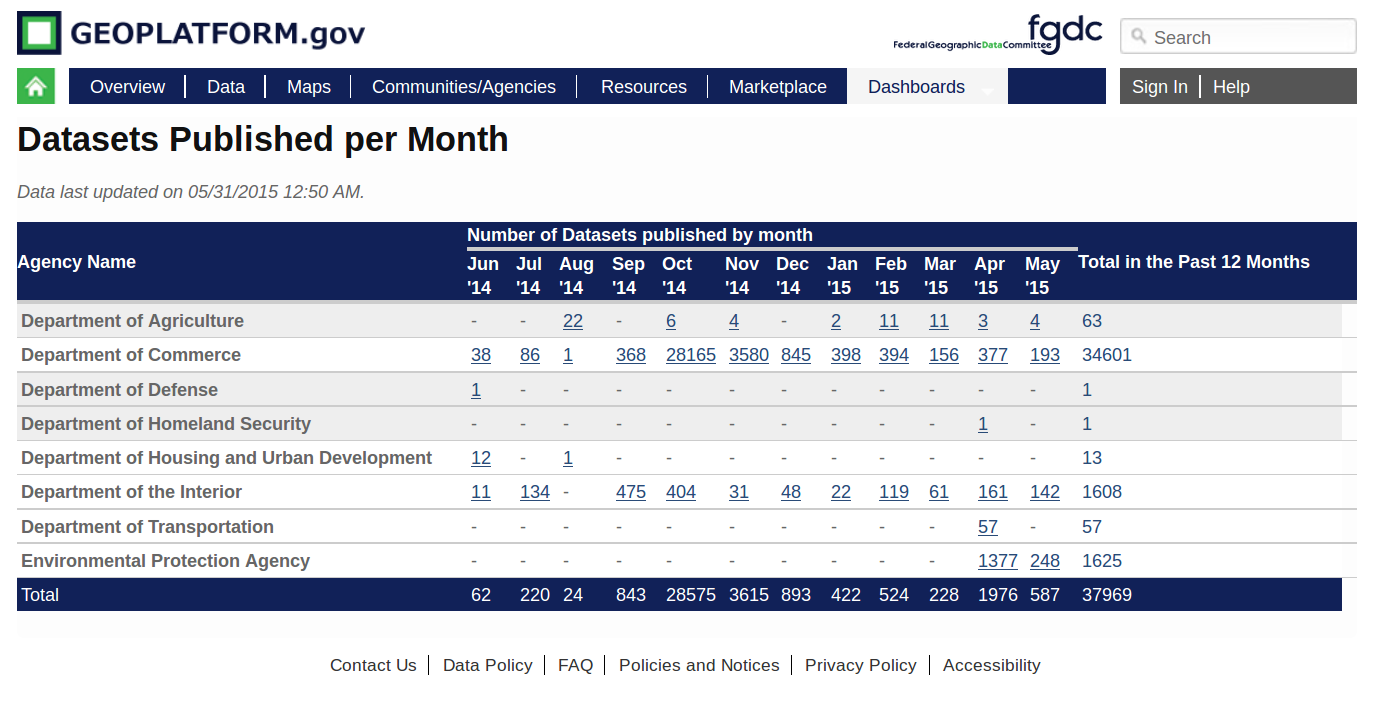
\includegraphics[width=\textwidth]{./images/GeoPlatform.png}
    \caption{Datasets publicados por Geoplatform}
  \end{figure}    

  \paragraph{La implementación de esta plataforma fue motivada por los principios y espirito de ``Open Government''\cite{21}, cuya principal visión es la de enfatizar la comunicación, contabilidad y transparencia entre gobierno-ciudadano, dentro del territorio estadounidense. Todos los datos, aplicaciones y servicios que provee Geoplatform se encuentran bajo licencias libres.}
  \paragraph{La plataforma fue desarrollada por miembros de la el comité federal de datos geográficos (FGDC por sus siglas en inglés) mediante la coolaboración de escuelas y usuarios expertos en el área. La audiencia que toma como fuente incluye agencias federales, estatales y locales, además de sector privado, educativo y al público en general. \cite{19}}
  \subsection{GeoMap México}
    \paragraph{GeoMap es una Plataforma Geoespacial Integral, que aprovecha las tecnologías informáticas actuales, implementando metodologías y estándares internacionales. Contiene todas las funcionalidades de un Sistema de Información Geográfica (SIG) y ofrece todos los servicios necesarios para la creación de aplicaciones geoespaciales.  Entre sus principales funcionalidades se encuentran: }
    \begin{itemize}
      \item Multiplataforma (Versión Escritorio, Web y para Dispositivos Móviles).
      \item Módulo de Mapas Dinámicos.
      \item Interacción con diferentes Servidores de Mapas.
      \item Conexión a distintas Bases de Datos Geoespaciales.
      \item Importación e Integración de información geográfica de diferentes fuentes y formatos.
      \item Visualización de Imágenes de Satélite, Ortofotos y de UAV (Vehículo Aéreo No Tripulado).
      \item Módulo de Administración y Autenticación de Usuarios. 
    \end{itemize}
    \paragraph{La plataforma Informática responde a la necesidad cada vez más frecuente de utilizar mapas y servicios geográficos en aplicaciones Web y para la Nube. Incluye las funcionalidades de integración y administración de información cartográfica, visualización y procesamiento de información geográfica y tabular, conexión a bases de datos geoespaciales e implementación de análisis espacial avanzado. La plataforma se especializa en temas como la geocodificación y geolocalización, áreas de influencia, zonas de cobertura, ubicación de puntos de interés, visualización, búsqueda y análisis de datos geográficos.}
    \begin{figure}[h!]
      \centering
        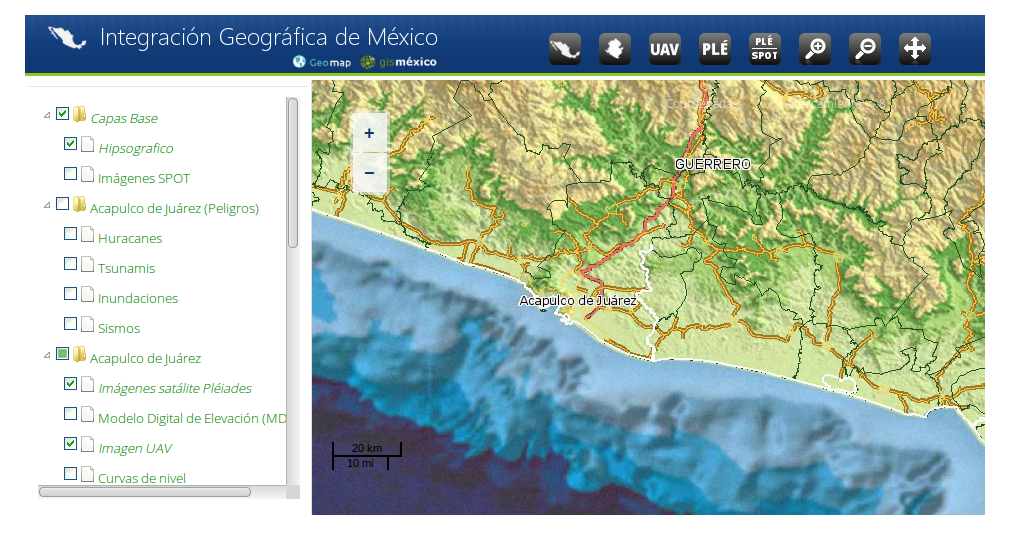
\includegraphics[width=\textwidth]{./images/GeoMap.png}
      \caption{Información publicada por GeoMap}
    \end{figure}
\section{Características climáticas y de contaminación en México.}
  \subsection{¿Cuándo se iniciaron los problemas de contaminación del aire?}
    \paragraph {Desde siempre la humanidad ha emitido contaminantes al aire, pero esto se incrementó de manera dramática a partir de la Revolución Industrial iniciada en el Reino Unido a finales del siglo XVII. En esa época, el trabajo manual fue remplazado por maquinaria, básicamente por la introducción de tecnologías que empleaban el vapor y que hacían posible tener altos niveles de producción. El problema fue que con estos avances industriales se incrementó el  uso de combustibles, tal como el petróleo y el carbón mineral, ambos indispensables para el funcionamiento de la nueva maquinaria.}

    \paragraph {Desde entonces el problema de contaminación del aire se ha convertido en una constante en muchas ciudades industriales de todo el mundo, lo que ha ocasionado problemas de salud a su población.}

    \paragraph {Algunos de los casos más dramáticos y graves son la famosa niebla tóxica londinense de 1952, el deterioro de los bosques europeos por la lluvia ácida en los años cincuenta y sesenta del siglo XX, y la grave situación de la calidad del aire en la Ciudad de México, Tokio y Sao Paulo durante las últimas décadas del siglo anterior. }

  \subsection {¿Cuáles son los contaminantes y qué efectos tienen?}
    \paragraph {Los contaminantes pueden ser emitidos de forma natural o por actividades relacionadas con el ser humano. Los fenómenos naturales que se producen en la superficie o  en el interior de la tierra –como el caso de erupciones volcánicas, que produce emisiones de gases, vapores, polvos y aerosoloes-, también contribuyen a la contaminación del aire.}
    
    \paragraph {Los principales contaminantes relacionados con la calidad del aire son el bióxido de azufre (SO2), el monóxido de carbono (CO), los óxidos  de nitrógeno (NOx), las partículas suspendidas, el plomo y el ozono.}
  
    \begin{figure}[h!]
      \centering
       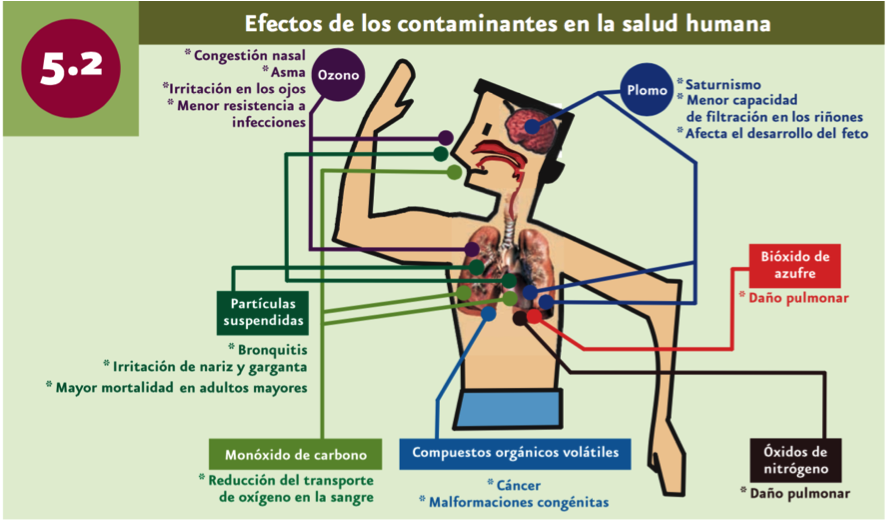
\includegraphics[width=12.5cm,height=9cm]{./images/1.png}
       \caption{Efectos de los contaminantes en el cuerpo.}
    \end{figure}

    \paragraph {Las plantas, animales y otros organismos también resienten los efectos de contaminantes como el ozono. Principalmente con la formación de la lluvia ácida, dicha lluvia es ocasionada con la presencia de ciertos ácidos en la atomósfera que se precipitan a la tierra con la lluvia. El dióxido de azufre y los óxidos de nitrógeno, resultado de la quema de combustibles  fósiles causan lluvia ácida, ya que al combinarse con agua, oxígeno y otros compuestos químicos forman ácidos como el ácido sulfúrico y el nítrico. }
    \paragraph{Las plantas se ven afectadas por esta lluvia ya que los ácidos pueden obstruir y acidificar los diminutos poros de las hojas por los que las plantas toman el aire que necesitan para realizar la fotosíntesis, además la lluvia ácida degrada los suelos, lo cual afecta las raíces y la nutrición de las plantas.}
  
    \paragraph {En el parque nacional Izta-Popo, Zoquiapan y en el Parque Nacional Desierto de los Leones, la lluvia ácida a dañado la vegetación. Estos daños involucran la pérdida de hojas y ramas, crecimiento lento y vulneravilidad a ataques de plagas y enfermedades.}
  
    \paragraph {Por otro lado los ríos, lagos y lagunas también pueden hacerse más ácidos por efecto de la lluvia ácida, lo cual pone en serio riesgo a las especies de plantas y animales que los habitan. Algunos ejemplos de estos daños se encuentran en los lagos del norte de Europa, en los que se ha reportado inclusio que han quedado sin ninguna forma de vida luego de la contaminación por lluvia ácida.}

    \begin{figure}[h!]
      \centering
        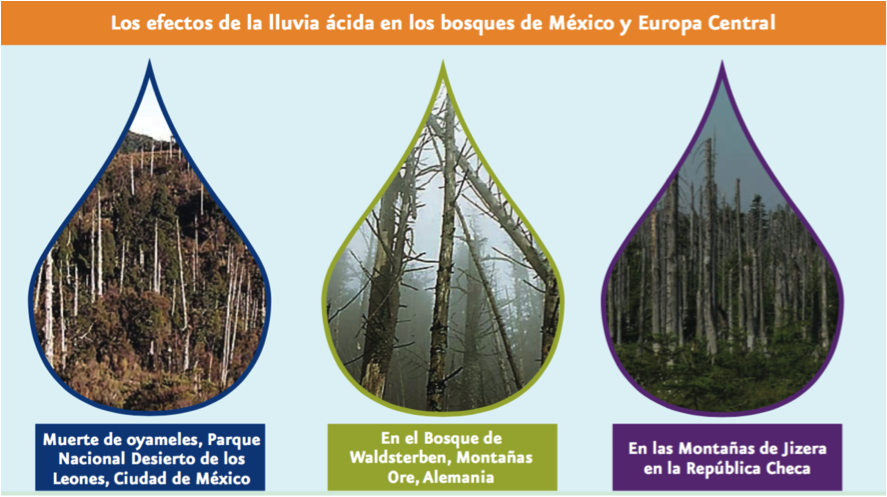
\includegraphics[width=\textwidth]{./images/2.png}      
      \caption{Impacto de la lluvia ácida en los bosques de México.}
    \end{figure}    

    \paragraph {Por otro lado también los monumentos y edificios sufren deterioros por la lluvia ácida, ya que los ácidos funcionan como agente corrosivo. El laboratorio de restauración del Instituto de Investigaciones Antropológicas de la UNAM indica que en losúltimos 25 años el deterioro de los monumentos y edificios históricos de la ciudad de México se ha acelerado de manera impresionante por el incremento de los niveles de contaminación.}

    \begin{figure}[h!]
      \centering
        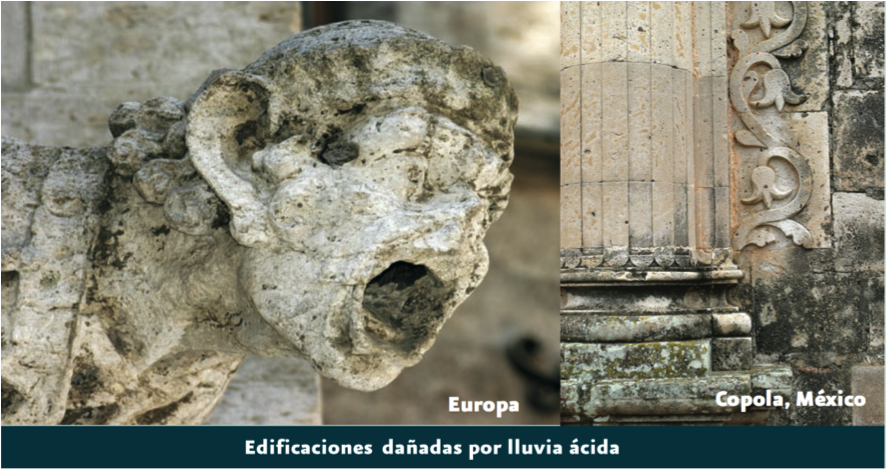
\includegraphics[width=\textwidth]{./images/3.png}
      \caption{Daños en edificaciones por lluvia ácida.}
    \end{figure}

  \subsection {Quiénes generan los contaminantes atmosféricos?}
    \paragraph {En México al igual que  en otros países se han desarrollado inventarios de emisiones que proporcionan información sobre la cantidad de contaminantes que se liberan al aire. En el año de 1999 de acuerdo al inventario de emisiones a nivel nacional se produjeron 40.5 millones de toneladas de las cuales el 58\% correspondieron a fuentes naturales- es decir, el suelo, la vegetación y las actividades volcánicas-    y 42\% a la contaminación de origen humano.}

    \paragraph {A pesar de que aparentemente las fuentes naturales sean las mayores productoras de contaminación, son las fuentes antropogénicas las que están cerca de la población y las que influyen en mayor medida en la calidad del aire que se respira.}

    \paragraph {Dentro de las fuentes antropogénicas, los vehículos automotores son los mayores productores de contaminantes, después la quema de gas LP y al final las emisiones de plantas generadoras de  electricidad.}

  \subsection {¿Qué hemos hecho para resolver el problema?}
    \paragraph {México lleva tiempo tomando acciones para resolver estos problemas, en 1988 implementó el Sistema Nacional del Inventario de Emisiones de Fuentes Fijas, así como un proyecto para cuantificar las emisiones del Valle de México. A partir del monitoreo de la calidad del aire ha diseñado algunas mejoras como eliminar el plomo en la gasolina, reducción del contenido de azufre.}

    \paragraph {Actualmente también existe una red de monitoreo atmosférico que abarca 52 ciudades y zonas metropolitanas que mide los niveles de contaminación presentes en el país. La concentración de los contaminantes en el aire se obtiene mediante la toma de muestras de aire que se analizan y procesan.}

    \paragraph {A partir de estas mediciones nacionales se han detectado cuales son las localidades con mayor índices de contaminación así como los contaminantes que emiten principalmente.  Uno de los esfuerzos más notables son los programas para mejorar la calidad del aire (Proaires) que buscan revertir las tendencias de deterioro, ya que incoroporan medidas para el control y abatimiento de las emisiones de los contaminantes.  También existen centrales eólicas para generar electricidad a partir de la energía del viento, una en la Venta, Oaxaca y la otra en Guerrero Negro, Baja California Sur.}  
  \clearpage
\chapter{Metodologías}

\section{Desarrollo ágil de software}
  \paragraph{El desarrollo ágil propone una alternativa al desarrollo de software tradicional. Los enfoques del desarrollo ágil son principalmente usados en el desarrollo de software para ayudar a las compañias a responder fácilmente al cambio.}

\subsection{Scrum}
  \paragraph{Scrum es un marco de gestión para el desarrollo incremental de un producto que proporciona una estructura de roles, reuniones, reglas y artefactos.}
  \paragraph{Scrum utiliza iteraciones de longitud fija denominados Sprints, que son típicamente de dos semanas o 30 días de duración. Los equipos de Scrum intentan generar un incremento de producto potencialmente entregable (debidamente probado) en cada iteración.}
  
 \subsection{Programación Extrema (XP)}
  \paragraph{Es un enfoque disciplinado para entregar software de alta calidad rápida y continuamente. Promueve una alta participación del cliente, retroalimentación rápida, pruebas continuas, planeación continua y entrega de software funcional en intervalos muy frecuentes que van de 1 a 3 semanas.}
  
\section{Técnicas de desarrollo ágil}

\subsection{Desarrollo guiado por pruebas (Test Driven Development)}


\section{Justificación}

A lo largo del desarrollo del proyecto se utilizarán prácticas características de varios frameworks y metodologías para el desarrollo ágil.

Principalmente plantearemos las historias de usuario que describan los flujos principales de la aplicación y posteriormente desarrollaremos entregables funcionales en plazos de tiempo conocidos como sprints en donde asignaremos un conjunto de actividades a cada integrante del equipo. Se realizará cada módulo utilizando siguiendo el desarrollo guiado por pruebas para asegurar la calidad del software. 



  \clearpage
\chapter{Tecnologías}
\section{Ventajas y Desventajas}

\begin{center}
  \begin{tabular}{ | c | p{6cm} | p{6cm} | }
    \hline
    Nombre & Ventajas & Desventajas \\
    \hline
    MongoDB & \tabitem Implementa funciones espaciales para encontrar información relevante de ubicaciones específicas. & \tabitem Difícultad para dar seguimiento a los cambios ya que la estructura de la base cambia constantemente. \\
            & \tabitem Útil para el procesamiento de grandes cantidades de información. & \\
    \hline
    Groovy & \tabitem Lenguaje expresivo. & \\
           & \tabitem Se pueden integrar fácilmente todas las bibliotecas de Java ya que corre sobre la JVM. & \\
           & \tabitem Closures & \\
    \hline
    Gradle  & \tabitem Sigue un enfoque de construcción por convención. & \tabitem La curva de aprendizaje es pronunciada si no se han utilizado antes herramientas como Ant o Maven \\
            & \tabitem Utiliza un poderoso lenguaje específico de dominio. (Groovy) & \\
            & \tabitem Cuenta con un administrador de dependencias que se encarga de 
                       descargarlas y las deja disponibles para su uso en la aplicación. & \\
    \hline

    Gulp  & \tabitem  Permite la automatización y ejecución de tareas para la construcción de un proyecto JavaScript.& \\
    \hline
   
  \end{tabular}
\end{center}

\clearpage
\begin{center}
  \begin{tabular}{ | c | p{6cm} | p{6cm} | }
    \hline
    Yeoman & \tabitem Define la estructura de directorios y archivos para un proyecto JavaScript & \\
           & \tabitem Cuenta con varios generadores para crear el código repetitivo que se necesita para iniciar un proyecto. & \\
           & \tabitem Define tareas para que el desarrollador se concentre sólo en realizar la funcionalidad de la aplicación. & \\
    \hline
    Ember & \tabitem Incrementa la productividad al desarrollar aplicaciones single page. & \tabitem Curva de aprendizaje muy pronunciada. \\
          & \tabitem Ember Data. & \\
          & \tabitem & \\
    \hline
    PhantomJS & \tabitem Automatización del navegador para realizar pruebas funcionales. & \\
              & \tabitem Opción para hacer screenshots de algún flujo de la aplicación. & \\
    \hline

  \end{tabular}
\end{center}

  \clearpage
\chapter{Modelo de Datos}

\section{Justificación}
\paragraph{Se hará uso de un modelo de base de datos orientado a documentos. También se contará con un esquema no relacional, es decir, se carece de una normalización definida, haciendo uso de  MongoDB, que se encargará de persistir y manejar las estructuras de datos en documentos JSON. Esta base de datos pertenece a la categoria NoSQL.}
\paragraph{ Las características de una base de datos NoSQL son las siguientes: }

\begin{itemize}
  \item Modelo de datos flexible.
  \item Buen rendimiento en clusters. 
  \item Sin esquemas.
\end{itemize}

\paragraph{Este tipo de bases resultan útiles debido a que se se pretende procesar grandes volúmenes de información para mostrar un historial de la información climática que se vaya persistiendo.}

\paragraph{Las tecnologías para grandes volumenes de información son relativamente nuevas; estas surgieron debido a la necesidad que tenían empresas grandes como Google y Amazon.} 

\paragraph{La información fue convertida de un modelo relacional a un modelo basado en documentos, jerárquico o basado en columnas usando proceso de denormalización, ésto con la finalidad de dar un orden a la información considerando simplemente consultas de cierto tipo evitando así operaciones típicas del álgebra relacional cómo el Producto Cartesiano, que implicaba el uso de grandes recursos.}

\paragraph{Las tecnologías de tipo NoSQL se orientan a consultas y no a transacción. Lo que brinda un fácil acceso a la información, una estructura de los datos orientada a su posterior análisis, respuestas en tiempo real y una gran capacidad de escalar y replicar. \cite{10}}

\paragraph{Empresas cómo Foursquare, Google, Amazon, Uber o Twitter, han optado por complementar la información que persisten de forma relacional con modelos orientados a documentos usando tecnologías como Hbase, MongoDB, BigTable, DynamoDB, por citar algunos ejemplos. \cite{11} \cite{12} }

\section{Descripción}
\paragraph{Considerando la problematica y solución que plantea el equipo de Ambienta2MX, se ha optado por orientar el sistema a consultas usando documentos como modelo de datos base. }

\paragraph{La información que será guardada y posteriormente consultada por otros módulos del ecosistema Ambienta2MX seguirá un esquema propuesto por el equipo de trabajo, éste recopila la estructura de sistemas que proveen información climática cómo lo son weather.gov, forecast.io, Weather Underground, proyecto INSPIRE (Unión Europea), Servicio Meteorológico Nacional, entre otros. \cite{13} \cite{14} \cite{15} }

\paragraph{Para la persistencia de la información se han definido los siguientes documentos:}
\begin{itemize}
  \item Places
  \item Pollution
  \item Weather  
\end{itemize}

\paragraph{Los documentos serán almacenados en MongoDB considerando los datos definidos en la especificación JSON Data Interchange Format (en su versión 2013). \cite{16}}

\paragraph{El equipo de Ambienta2MX ha considerado el uso de el formato antes mencionado debido a su facilidad de lectura e integración con otro tipo de plataformas y lenguajes de programación, actualmente es el formato que rige el manejo de API de tipo REST.}

\paragraph{Dentro de los modelos existe información relativa a los proveedores o fuentes de información, ésta información será utilizada para fines de consulta y contar con el control del origen de los datos.}
\newpage
\subsection{Places}
  \lstinputlisting[language=Javascript]{../Resources/PlacesDoc.js} 
\newpage
\subsection{Pollution}
  \lstinputlisting[language=Javascript]{../Resources/PollutionDoc.js} 
\newpage
\subsection{Weather}
  \lstinputlisting[language=Javascript]{../Resources/WeatherDoc.js} 


  \chapter {Definici\'on tem\'atica de Ambienta2MX}
  \section {Objetivo general}
    \paragraph {Considerando el problema de informaci\'on y estructura de datos que tiene M\'exico en la actualidad, adem\'as de seguir la tendencia y aprovechar la brecha que ha disminuido el uso de datos abiertos, el equipo de \underline{Ambienta2MX} decidi\'o afrontar la tarea de desarrollar una herramienta que permita la conceptualizaci\'on de la informaci\'on de variables ambientales e indices de calidad y contaminaci\'on del aire que el INEGI y otras instituciones p\'ublicas o privadas almacenan y/o exponen para fines educativos, informativos o de uso part\'icular.}
  
  \section{Justificación}
    \paragraph{Existe la necesidad de una fuente de datos que presente información climática}
  \chapter {Descripción y Módulos de Ambienta2MX}
  \section {¿Qué y para qué es Ambienta2MX?}
    \paragraph {\underline{Ambienta2MX} es el nombre de la plataforma que formará parte de una macro solución orientada a la estandarización de metadatos que el INEGI y otras instituciones públicas.}
    \paragraph{Actualmente no existe un estándar de datos geográficos a nivel nacional. Han existido aproximaciones mediante concursos que instituciones públicas como el INEGI ha publicado, o simplemente han existido propuestas que han brindado una solución incompleta a la unión y manejo de información geográfica, geodésica, hidrográfica, climática, topográfica, etc.}
    \paragraph{\underline{Ambienta2MX} toma parte de todo el problema y propone una infraestructura lógica para afrontar la estandarización de variables ambientales y algunos índices de contaminación. Esta información actualmente se encuentra en formatos muy rudimentarios como textos planos sin algún protocolo o formato de interpretación.}
    \paragraph{Sistemas semejantes, por ejemplo, el \textbf{Servicio Meteorológico Nacional} carece de algún recurso del cual se puedan realizar consultas que no sea mediante su portal web, esto trae problemas directos de compatibilidad con otros sitemas. Un caso semejante tenemos con la información que la \textbf{Conagua} maneja en sus centrales meteorológicas a lo largo del país, los datos que brindan se actualizan de forma periodica y el único medio de acceso es a través de una página de internet que devuelve archivos en formato de texto u hojas de cálculo.}
    \paragraph{Los impedimentos antes mencionados conllevan a situaciones tan triviales como la consulta de datos para algúna región o punto específico del territorio nacional, al existir diversas fuentes no es posible tener un compendio del cual tomar la información que más nos convenga. Si a este problema se le añade que los datos carecen de un estandar, llegamos al punto en el que intentar manipular o tratar los datos se vuelve una tarea complicada y en exceso tediosa.}
    \paragraph{Considerando dichos problemas \underline{Ambienta2MX}, propone un estandar de datos climáticos tomando como referencia diversas fuentes y adaptando los tipos de datos a tecnologías y tendencias actuales, brindando así una mayor portabilidad y simplicidad en la consulta de información.}
  \newpage
  \section{Diagrama de Ambienta2MX}
    \paragraph{\underline{Ambienta2MX} constará de varios módulos que trabajarán de forma conjunta para satisfacer la necesidad de tener un estandar y un repositorio de datos climáticos a nivel nacional.}
    \paragraph{Al brindar un sistema modularizado, se genera de forma directa un impacto en el proceso de análisis, desarolló e intengración. Éste tipo de modelo describe de una forma sencilla los componentes necesarios para solventar la demanda a la que se encontrará sometida la plataforma.}
    \paragraph{A continuación se muestra el diagrama a bloques de \underline{Ambienta2MX}, todos los módulos, recursos y bases de datos serán descritos de forma posterior.}
  \newpage
    \begin{landscape}
      \begin{figure}[h!]
      \centering
      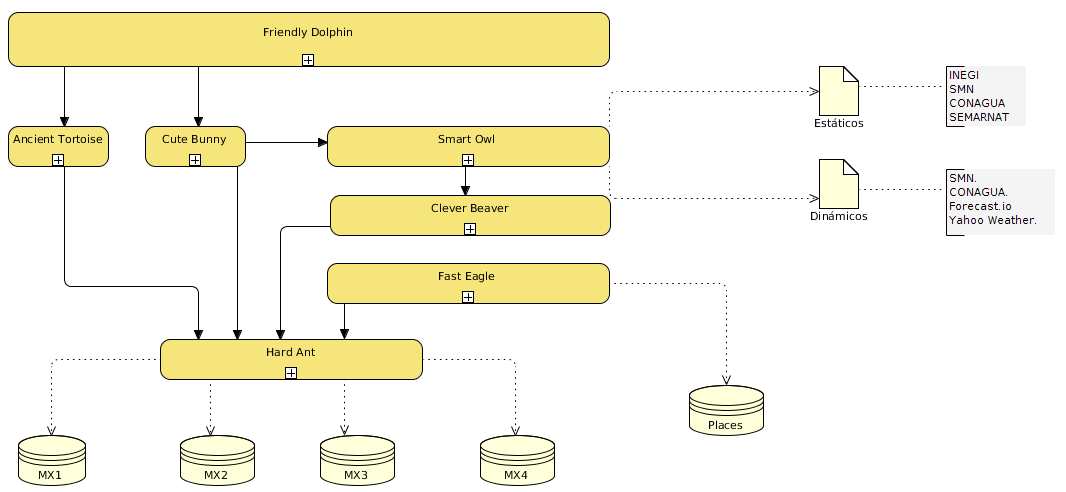
\includegraphics[width=22.5cm,height=12cm]{./images/DiagramaAmbienta2MX.png}
      \caption{Módulos y estructura de Ambienta2MX}
    \end{figure}
    \end{landscape}
  \newpage
    \paragraph{Cómo se apreciar en el diagrama, además de los gestores de bases de datos, \underline{Ambienta2MX} se encuentra dividido en siete módulos básicos:}
    \begin{itemize}
    \item Friendy Dolphin.
    \item Ancient Tortoise.
    \item Cute Bunny.
    \item Smart Owl.
    \item Clever Beaver.
    \item Fast Eagle.
    \item Hard Ant.
  \end{itemize}
    \paragraph{En el mismo diagrama se pueden observar las fuentes que proporcionarán la información ya sea a un nivel estático, por ejemplo, carta climática anual de algún municipio del territorio nacional; o bien, recursos que se actualizan de forma periodica como son los datos que provee el Servicio Meteorológico Nacional.}
    \paragraph{Se condieran cinco bases de datos, \emph{MX1, MX2, MX3, MX4, Places}. Todas las bases del tipo MX contarán con la información de variables ambientales así también de los índices de contaminación de las zonas que conforman al territorio nacional.}
    \paragraph{Para el caso de \emph{Places}, la base será usada como un macro índice cartográfico del territorio nacional, es decir, esta base será la referencia a nivel latitud, longitud y altitud para ubicar los datos que requieran ser procesados.}
    \paragraph{Todas las bases se encontrarán funcionando bajo un modelo de base de datos documental teniendo una alimentación bajo demanda, es decir, el contenido gestionado irá aumentando conforme las éstos vayan siendo solicitados.}
\section{Módulos de Ambienta2MX}
  \subsection{Friendly Dolphin}
    \subsubsection{Definición}
      \paragraph{Éste módulo es el encargado de brindar la información procesada al usuario a través de una página de internet. Es el módo visual que los usuarios finales tendrán para poder interactuar con el ecosistema Ambienta2MX.}
      \paragraph{Se presenta cómo un módulo web que consumirá la información procesada y almacenada por las cuatro bases (MX1,MX2,MX3,MX4) y la base de soporte (Places).}
      \paragraph{La principal función es la de consulta y visualización de datos. Es la capa más expuesta y menos técnica de Ambienta2MX ya que es la que tendrá interacción directa con usuarios no técnicos, sin embargo, contará con los procesos necesarios para poder extraer información de las demás plataformas en formatos convencionales cómo JSON, XML o CSV para uso posterior del usuario.}
      \paragraph{Interactua de forma directa con los bloques \textbf{\emph{Ancient Tortoise}} y \textbf{\emph{Cute Bunny}}, que forman parte de la segunda capa de exposición de datos de Ambienta2MX. Se comunica con los demás módulos mediante servicios de tipo REST que funcionan bajo el patrón de convención sobre configuración\cite{8}, brindando así una gran compatibilidad con éstos además de mejorar el tiempo de desarrollo debido a que no es necesario generar código único y se opta por la reutilización de código y bibliotecas que siguen el mismo método de trabajo.}
  \subsubsection{Diagrama por bloques}
   \paragraph{Friendly Dolpin contará con varios procesos y módulos a ser desarrollados. Éste módulo se desarrollará usando tecnologías cómo HTML, Javascript y CSS, además de contar con un ciclo continuo de desarrollo usando herramientas de apoyo cómo Yeoman, Gulp para el maquetado y gestión de tareas comunes en projectos de tipo web. A continuación se muestra el diagrama básico de la aplicación.}
  \newpage
    \begin{landscape}
      \begin{figure}[h!]
      \centering
      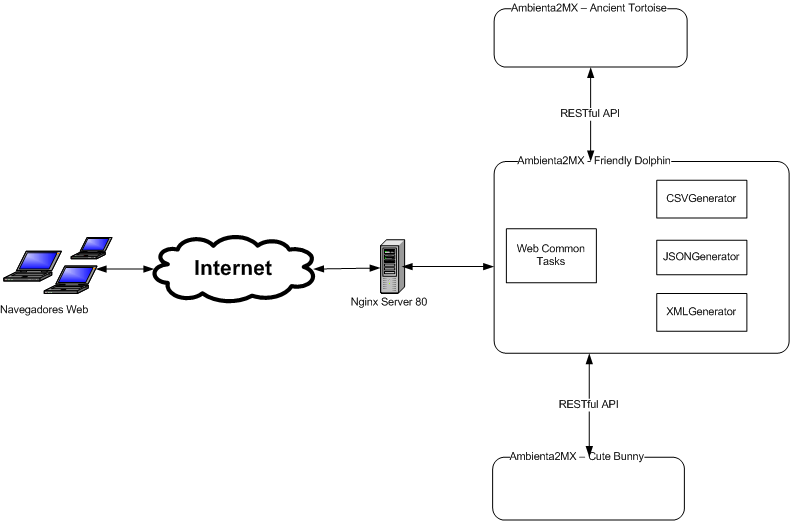
\includegraphics[width=22.5cm,height=12cm]{./images/DiagramaFriendlyDolphin.png}
      \caption{Diagrama General de Friendly Dolphin}
    \end{figure}
    \end{landscape}
  \newpage
  \paragraph{Las tecnologías a usar para este módulo serán basicamente Javascript, HTML y CSS. Usando el servidor interno que ofrece Gulp junto con las tareas y gestión de bibliotecas de terceros. En cuanto al desarrollo de los estilos necesarios para las vistas se implementará Bootstrap cómo maquetado CSS y finalmente el manejo de vistas, peticiciones y lógica dentro del navegador de los clientes se implementará usando EmberJs.}
  \subsection{Cute Bunny}
    \subsubsection{Definición}
     \paragraph{El módulo \textbf{\emph{Cute Bunny}} es parte medular para la comunicación con otros sistemas. Cute Bunny es el encargado de proporcionar los respectivos servicios de tipo REST a otros sistemas o módulos que deseen consultar la información almacenada en las respectivas bases de tipo MX.}
     \paragraph{La información de variables ambientales e índices de contaminación y calidad del aire, será expuesta por medio de peticiones HTTP que siguen un patrón Conv over Conf, es decir, sigue la misma estructura que otros sitemas y frameworks de desarrollo web, esto facilitará que aquellos desarrolladores y analistas que deseen acceder de forma programática no tengan que realizar demasiadas configuraciones y se adapten de forma orgánica al sistema.}
     \paragraph{Considerando la naturaleza del sistema, que es un sistema primordialmente de consultas y extracción de información de sistemas externos, no es necesario contar con una extensa lógica de negocio. El núcleo de la aplicación será la exposición de datos y seguir la convención de servicios REST, cómo muestra el siguiente diagrama.}
      \begin{figure}[h!]
        \centering
        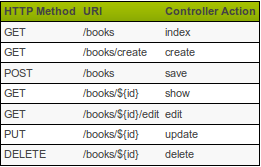
\includegraphics[width=5cm,height=3cm]{./images/DiagramaREST.png}
        \caption{Tabla de peticiones a Cute Bunny}
     \end{figure}
  \paragraph{Cute Bunny interactua con otros dos módulos de Ambienta2MX, Smart Owl y Hard Ant. La interacción con estos surge debido a que Hard Ant es el encargado de gestionar el acceso a las bases de datos de tipo MX y Smart Owl brindará y dará solución a las busquedas que no se encuentren en las bases de tipo MX, es decir, tratará de encontrar la información que Cute Bunny le solicitó para guardarla en algunas de las bases y posteriormente regresar el resultado al solicitante.}
      \begin{landscape}
        \subsubsection{Diagrama por bloques}
        \paragraph{A continuación se mostrará el diagrama por bloques que define la estructura de Cute Bunny.}
          \begin{figure}[h!]
          \centering
          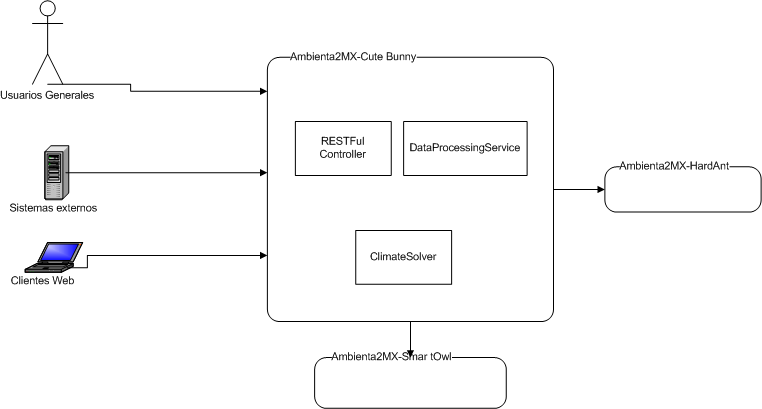
\includegraphics[width=22.5cm,height=12cm]{./images/DiagramaCuteBunny.png}
          \caption{Diagrama General de Cute Bunny}
        \end{figure}
      \end{landscape}
  \subsection{Ancient Tortoise}
    \subsubsection{Definición}
      \paragraph{El principal objetivo de este módulo es procesar y mostrar la información histórica de las variables almacenadas en las bases de datos de tipo MX. Ancient Tortoise tomará calculará y generará por medio de una regresión lineal una predicción, a lo más de un mes, de las variables ambientales y de contaminación de un estado o localidad en específico.}
      \paragraph{La información obtenida a demanda por el módulo Smart Owl será la fuente de información básica para generar los modelos de predicción necesarios. Éste no modificará la información existente en la base de datos, sólo obtendra la información y calculará los datos entre los rangos de fechas definidos por el usuario desde la interfaz generada en Friendly Dolphin.}
      \paragraph{El usuario final tendrá interacción con estas operaciones ya sea a través de un servicio REST o usando la interfaz web que proporciona Friendly Dolphin. El diagrama por bloques del módulo aisla el módulo de calculos matemáticos dejando sólo expuesto el servicio para consultas dado una localidad o estado de la Republica Mexicana considerando como límites una fecha inicial y final. El módulo proveerá la opción de exportar la información generada por éste en los formatos JSON y XML.}
      \begin{landscape}
      \subsubsection{Diagrama por bloques.}
        \paragraph{A continuación se mostrará el diagrama por bloques que define la estructura de Ancient Tortoise.}
        \begin{figure}[h!]
        \centering
        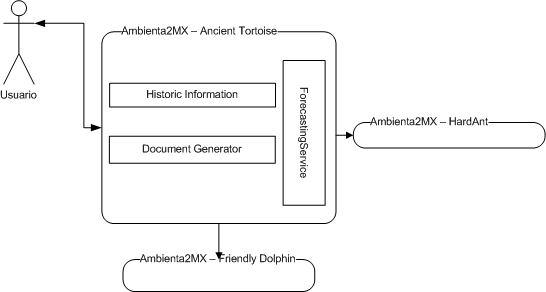
\includegraphics[width=22.5cm,height=12cm]{./images/DiagramaAncientTortoise.png}
        \caption{Diagrama General de Ancient Tortoise}
      \end{figure}
      \end{landscape}
  \subsection{Smart Owl.}
    \subsubsection{Definición}
      \paragraph{La función principal del Smart Owl es la obtención de la información de diversas fuentes, tanto estáticas y dinámicas. Todas la información que se encontrará en las bases de datos de tipo MX será obtenida a través de Smart Owl, muchas de las fuentes no cuentan con los datos climatológicos completos, principalmente las gubernamentales (CONAGUA, INEGI, SMN); considerando esa problematica, Smart Owl buscará y tratará de resolver la información de los campos faltantes tomando como base distintas fuentes de datos, algunas establecidas y otras de tipo gubernamental.}
      \paragraph{El modelo de datos final podrá ser entonces persistido después de que haya sido resuelto completa o parcialmente. Se llevará el control de los metadatos considerando la fuente de datos, su fecha y algunos tags relacionados con sus respectivas fuentes.}
    \subsubsection{Diagrama por bloques}
  \subsection{Clever Beaver}
    \subsubsection{Definición}
    \subsubsection{Diagrama por bloques}
  \subsection{Fast Eagle}
    \subsubsection{Definición}
      \paragraph{El módulo Fast Eagle formará parte de la arquitectura final de Ambienta2MX. El propósito principal de este módulo es brindar la información cartográfica de México por medio de un servicio expuesto, considerando latitud, longitud o nombre de la localidad deseada.}
      \paragraph{Fast Eagle se encargará de la lectura, carga, verificación y resolución de los archivos brindados por el (Instituto Nacional de Estadística y Geografía) INEGI en la información pública que tiene de la cartografía del territorio nacional.}
      \paragraph{La información que proporciona el INEGI carece de campos esenciales para la estandarización de los datos cartográficos, para dar solución a ese contratiempo se hará uso de servicios externos que ya cuentan con información definida, es decir, que su información ha pasado bajo un cierto proceso de limpieza y regulación, por ejemplo, los servicios de Google Places API y GeoHack.}
    \subsubsection{Diagrama por bloques}
      \paragraph{Fast Eagle contará con varios procesos a ser desarrollados, la integración de cada proceso y su respectiva integración dará solución a un problema de estandarización, resolución y consulta de datos geográficos vía Latitud, Longitud y Ubicación.}
    \newpage
      \begin{landscape}
        \begin{figure}[h!]
        \centering
        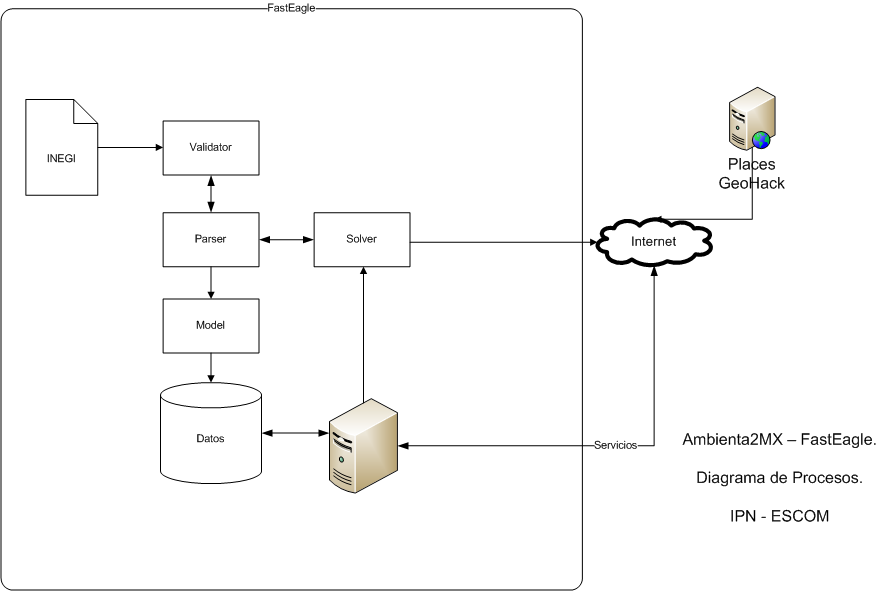
\includegraphics[width=22.5cm,height=12cm]{./images/DiagramaFastEagle.png}
        \caption{Diagrama General de Fast Eagle}
      \end{figure}
      \end{landscape}
    \newpage
    \paragraph{En el diagrama se muestran cuatro módulos básicos, estos forman parte del núcleo de Fast Eagle, también podemos observar que se cuenta con la interacción de servicios de terceros como Google Places y GeoHack, también se cuenta con la exposición de los servicios a través de un servidor  web.}
    \paragraph{El módulo de Validación \textbf{\emph{Validator}}, será el encargado de tomar las fuentes que el INEGI brinda al público en general en forma de archivos CSV, y realizar un proceso de validación a los datos que éstos tienen.}
    \paragraph{El módulo indicará que datos necesitan una resolución y cuáles pueden ser estandarizados y posteriormente almacenados en la base de datos.}
    \paragraph{\textbf{\emph{Parser}} tomará los datos que el proceso de validación le arroje para transformar al estado propuesto por el equipo de trabajo (Véase modelo de datos). Considerando un proceso de resolución en caso de que la información proporcionada por el INEGI se encuentre incompleta no sea válida.}
    \paragraph{Para toda la información que carezca de datos correctos \textbf{\emph{Solver}} buscará una resolución en servicios de terceros, después de la resolución, los datos serán guardados en el gestor de bases de datos bajo el formato propuesto por el equipo de trabajo.}
    \paragraph{\textbf{\emph{Model}} es la capa de interacción con la base de datos, ésta se encarga de las operaciones mejor conocidas como CRUD (Create, Read, Update and Delete),  persistiendo la información en MongoDB.}
    \paragraph{Para poder exponer los datos, se hará uso de un servidor web minimalista orientado a micro servicios, éste será un servicio público que formará parte de la infraestructura final de Ambienta2MX.}
    \paragraph{El servicio expuesto se encargará de las búsquedas a nivel base de datos y en caso de no encontrar la información buscará en terceros para poder agregarla a la base de datos y así ir mejorando el contenido de nuestro índice cartográfico.}
    \paragraph{Se usará Groovy y Vertx para el desarrollo de Fast Eagle, esto debido a la fácil integración entre los lenguajes y tecnologías, también debido a que se busca una gran escalabilidad y fácil soporte para la plataforma en caso de que ésta lo necesite.}
    \paragraph{Para la automatización de la ejecución de las pruebas, el proceso de compilación y despliegue del módulo así como para su ejecución se hará uso de Gradle que permite crear tareas a través del lenguaje de programación Groovy.}
  \subsection{Hard Ant}
    \subsubsection{Definición}
      \paragraph{Hard Ant es uno de los bloques funcionales base de Ambienta2MX, su función principal es la de enrutar las peticiones a las bases de tipo MX además de brindar la solución cartográfica (a nivel ubicación) interactuando con Fast Eagle. Hard Ant brindará los canales de acceso a las bases MX definidas en el diagrama general mediante servicios HTTP, estos servicios brindarán información para el proceso de inserción y extracción de la información. }
      \paragraph{Este módulo es lo que sería considerado la capa del modelo de datos en un patrón MVC, ya que es la que tiene contacto de forma directa con los datos almacenados en las bases de datos orientadas a documentos gestionadas por Mongo. Se utilizará un pool de conexiones a la base para garantizar el acceso o escritura a los datos además de brindar la posibilidad de respuestas asincronas y no bloqueantes entre las consultas realizadas.}
      \paragraph{Considerando trabajos más pesados (Obtención de datos históricos) se utilizarán procesos en segundo plano, esto es posible gracias a la implementación de ``Verticles'' nativas de Vert.x, tecnología que será usada para el desarrollo y despliegue final de éste módulo}
    \subsubsection{Diagrama por bloques}
      \newpage
        \begin{landscape}
          \begin{figure}[h!]
          \centering
          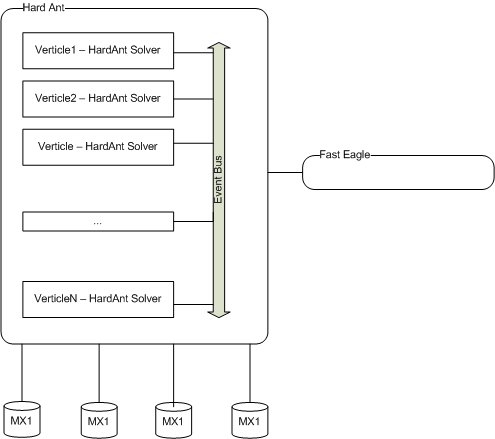
\includegraphics[width=22.5cm,height=12cm]{./images/DiagramaHardAnt.png}
          \caption{Diagrama General de Hard Ant}
        \end{figure}
        \end{landscape}
      \newpage
    \paragraph{En el diagrama se puede apreciar la replicación de ``Verticles'' que interactuan a través del mismo canal de información, esto brinda una alta disponibilidad del servicio ya que las peticiones son atendidas y procesadas no sólo por un elemento existente si no varios. Otros módulos de Ambienta2MX pueden conectarse a este canal de información ya sea de forma local o distribuida.}
  \subsection{Otros.}
    \subsubsection{Módulo de WebScrapping - Wicked Fox}
    \paragraph{Este módulo será el encargado de tomar información de plataformas que carecen de un servicio web definido, por ejemplo el Sistema Meteolorógico Nacional. Toda la información que exponen de forma diaria, semana, mensual y anual. Se encuentra bajo un formáto HTML que puede ser visualizado a través de algún navegador web al acceder a su sitio.}
    \paragraph{Problemas cómo los anteriores suelen ser comunes a nivel nacional (principalmente plataformas gubernamentales), para poder hacer uso de esos recursos es necesario generar un módulo que de forma programática pueda extraer limpiar, extraer y adecuar la información.}
    \paragraph{Al proceso antes descrito se le conoce cómo \emph{Web Scrapping}\cite{6}, que se define cómo la extracción de información de sitios web a través de medios programáticos o programas definidos.}
    \paragraph{Éste módulo se encuetra implementado bajo un script escrito en Javascript usando PhantomJs cómo medio lógico y programático para la implemtación del Scrapping.}
    \paragraph{ La definición básica de \textbf{\emph{Wicked Fox}} es tomar el recurso que brinda el SMN, extraer la información contenida en tablas y posteriormente mandar esta información al módulo \textbf{\emph{Smart Owl}} que se encargará de adecuar y después delegar el trabajo al módulo de registro masivo \textbf{\emph{Clever Beaver}} donde al final la información climatológica de cierta localidad será guardad en alguna de las bases de datos antes mencionadas.}
      \begin{landscape}
        \begin{figure}[h!]
        \centering
        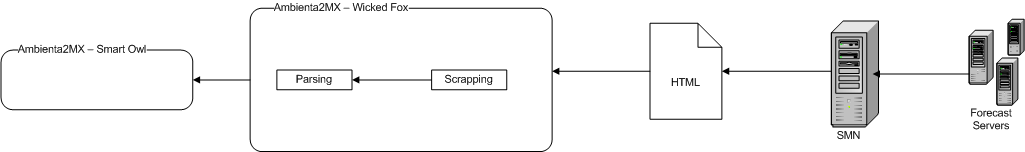
\includegraphics[width=11cm,height=6cm]{./images/DiagramaWickedFox.png}
        \caption{Diagrama General de Wicked Fox}
      \end{figure}
      \end{landscape}
    \paragraph{Éste módulo presenta una gran importancia debido a que actualmente se carece de un servicio a nivel nacional que brinde información meteorológica con cierta veracidad, si bien es cierto que otros sistemas extraen información de datos tomados por centrales mexicanas, el costo de éstos suele ser elevado.}
    \paragraph{La extracción de la información se ejecutará \emph{al vuelo}, es decir, éste proceso se ejecutará cada que se pidan datos con un margen no mayor a una hora de cierta localidad o ubicación del territorio nacional.}
    \paragraph{Para poder hacer uso de éste módulo es necesario brindar la información de la localidad via latitud/longitud o bien, a través de la localidad descrita, éstos datos serán proporcionados y resueltos por el módulo \textbf{\emph{Fast Eagle}} descrito anteriormente.}
  \chapter {Glosario}
    \begin{itemize}
		\item \textbf{JSON}: Javascript Object Notation, Es un formato ligero de intercambio de datos.
		\item \textbf{ITRF}: Acrónimo de International Terrestrial Reference System (Marcos de Referencia Terrestre Internacional).
		\item \textbf{NAD27}: Acrónimo de North American Datum of 1927. Marco de referencia terrestre usado por el INEGI hasta el año 1998.
		\item \textbf{GIS}: Sistema de Información Geográfica.
    \item \textbf{API}: Application Programming Interface, conjunto de rutinas, protocolos o herramientas para construcción de software.
    \item \textbf{REST}: Representational State Transfer, Arquitectura de sofware para sistemas web basada en un patrón ``Convention over configuration'' con operaciones que funciona usando el protoclo HTTP como base.
	\end{itemize}
  \begin{thebibliography}{1}
	\bibitem{1}
		Mapa Digital de México, INEGI 2014, Available at: \url{http://gaia.inegi.org.mx/mdm6/}
	\bibitem{2}
	   Modelo de datos CIM, 2013, Available at: \url{https://earthsystemcog.org/projects/es-doc-models/cim}
	\bibitem{3}
		 GIS México - Sistemas de Información Geográfica, Available at: \url{http://www.sigmexico.com.mx/}
	\bibitem{4}
	     GEOJson Format Specification, 2008, Available at: \url{http://geojson.org/geojson-spec.html}
	\bibitem{5}
		 GIS (Geographic information system), 2010, Available at: \url{http://education.nationalgeographic.com/education/encyclopedia/geographic-information-system-gis}
	\bibitem{6}
		INEGI, Acerca del INEGI, N/A, Available at: \url{http://www.inegi.org.mx/inegi/acercade/default.aspx}
	\bibitem{7}
		Web Scrapping Introduction, Geoff Boeing, Berkeley University, 2014, Available At: \url{http://dlab.berkeley.edu/sites/default/files/training\_materials/web-scraping-talk.pdf}
	\bibitem{8}
		Convention over configuration, Microsoft Developers Network, 2012, Available At: \url{https://msdn.microsoft.com/en-us/magazine/dd419655.aspx}.
	\bibitem{9}
	    INSPIRE Project, Aboute INSPIRE, Available at: \url{http://inspire.ec.europa.eu/}
	\bibitem{10}
		NoSQL Explained, MongoDB Courseware, Available at: \url{https://www.mongodb.com/nosql-explained}
	\bibitem{11}
		Seven databases in seven weeks: A guide to Modern Databases and NoSQL movement, Eric Redmond, Pragmatic Bookself, 2013.
	\bibitem{12}
		MongoDB Case Study: Foursquare, Mongodb Courseware, Available at: \url{http://www.mongodb.com/post/15400944604/mongodb-case-study-foursquare}
	\bibitem{13}
		Weather Underground, About the Data, Available at: \url{http://www.wunderground.com/about/data.asp}
	\bibitem{14}
		Forecast.io, Data Sources, Available at: \url{http://forecast.io/raw/}
	\bibitem{15}
		Servicio Meteorológico Nacional, Conceptos, Available at: \url{http://smn.cna.gob.mx/index.php?option=com_content&view=article&id=23&Itemid=120}
  \bibitem{16}
    The JSON Data Interchagnge Format, ECMA International, 2013, Available at: \url{http://www.ecma-international.org/publications/files/ECMA-ST/ECMA-404.pdf}
\end{thebibliography}
\end{document}
